\documentclass{article}
\usepackage[utf8]{inputenc}
\usepackage[T1]{fontenc}
\usepackage{graphicx}
\usepackage{amsmath, amssymb}
\usepackage{xcolor}
\usepackage{tikz}
\usepackage{enumitem}
\usepackage{lipsum}
\usetikzlibrary{fit}
\usepackage{hyperref} 
\usepackage{subfig}
\usepackage{xcolor}
\usepackage{colortbl}

% Define colors
\definecolor{lessoncolor}{RGB}{74, 144, 226}
\definecolor{examplecolor}{RGB}{92, 184, 92}
\definecolor{notecolor}{RGB}{255, 179, 102}

% Define a command for colorful sections
\newcommand{\colorsection}[1]{\section*{\textcolor{lessoncolor}{#1}}}

% Set up TikZ for graphing
\usetikzlibrary{positioning, arrows.meta, shapes.geometric}

% Document
\begin{document}

\begin{titlepage}
    \centering
    \vspace*{2cm}
    {\LARGE \textcolor{lessoncolor}{Advanced Functions}}\par
    \vspace{1cm}
    {\large Your Name}\par
    \vspace{2cm}
    {\large \today}\par
    \vspace{3cm}
\end{titlepage}
\tableofcontents
\newpage


\section*{Review}
\subsection{Exponent Laws}
 
\subsubsection*{Product Law}
When multiplying two terms with the same base, add the exponents.
\[ a^m \cdot a^n = a^{m + n} \]

\subsubsection*{Quotient Law}
When dividing two terms with the same base, subtract the exponents.
\[ \frac{a^m}{a^n} = a^{m - n} \]

\subsubsection*{Power Law}
When raising a power to another power, multiply the exponents.
\[ (a^m)^n = a^{mn} \]

\subsubsection*{Zero Exponent Law}
Any nonzero number raised to the power of zero is equal to 1.
\[ a^0 = 1 \]

\subsubsection*{Negative Exponent Law}
\[ a^{-n} = \frac{1}{a^n} \]
\newpage
\subsection{Common Number Sets}

\subsubsection*{Natural Numbers ($\mathbb{N}$)}
The set of natural numbers is denoted by $\mathbb{N}$ and includes all positive integers from 1 onwards. 
\[ \mathbb{N} = \{1, 2, 3, 4, \ldots\} \]

\subsubsection*{Integers ($\mathbb{Z}$)}
The set of integers is denoted by $\mathbb{Z}$. It includes all whole numbers, both positive and negative, including zero.
\[ \mathbb{Z} = \{\ldots, -3, -2, -1, 0, 1, 2, 3, \ldots\} \]

\subsubsection*{Rational Numbers ($\mathbb{Q}$)}
The set of rational numbers is denoted by $\mathbb{Q}$. It includes all numbers that can be expressed as a fraction of two integers, where the denominator is not zero.
\[ \mathbb{Q} = \left\{\frac{a}{b} \mid a,b \in \mathbb{Z}, b \neq 0\right\} \]

\subsubsection*{Real Numbers ($\mathbb{R}$)}
The set of real numbers is denoted by $\mathbb{R}$. It includes all rational and irrational numbers, forming the continuum on the number line.

\subsubsection*{Complex Numbers ($\mathbb{C}$)}
The set of complex numbers is denoted by $\mathbb{C}$. It includes all numbers of the form $a + bi$, where $a$ and $b$ are real numbers and $i$ is the imaginary unit.

\begin{figure}[ht]
    \centering
    \includegraphics[width=0.35\textwidth]{imgs/number-sets-nzqar.jpg}
    \end{figure}

\newpage    
\section{Unit 1}
\subsection{Power Functions}

\begin{minipage}[t]{\textwidth}
Linear and Quadratic functions are the two most encountered polynomial functions. Polynomials are defined as follows...

A polynomial expression is an expression of the form
\[
a_n x^n + a_{n-1} x^{n-1} + a_{n-1} x^{n-2} + \ldots + a_3 x^3 + a_2 x^2 + a_1 x + a_0,
\]
where
\begin{itemize}
    \item \( n \) is a whole number
    \item \( x \) is a variable
    \item the coefficients \( a_0, a_1, \ldots, a_n \) are real numbers
    \item the degree of the function is \( n \), the exponent of the greatest power of \( x \)
    \item \( a_v \), the coefficient of the greatest power of \( x \), is the leading coefficient
    \item \( a_0 \), the term without a variable, is the constant term
\end{itemize}

A polynomial function has the form
\[
f(x) = a_n x^n + a_{n-1} x^{n-1} + a_{n-2} x^{n-2} + \ldots + a_5 x^3 + a_2 x^2 + a_1 x + a_0
\]

Power functions, the simplest polynomial functions, have one term and transform into a general polynomial function when transformed.
\end{minipage}

\vspace{0.5cm}

\begin{center}
\begin{minipage}[t]{0.8\textwidth}
\centering
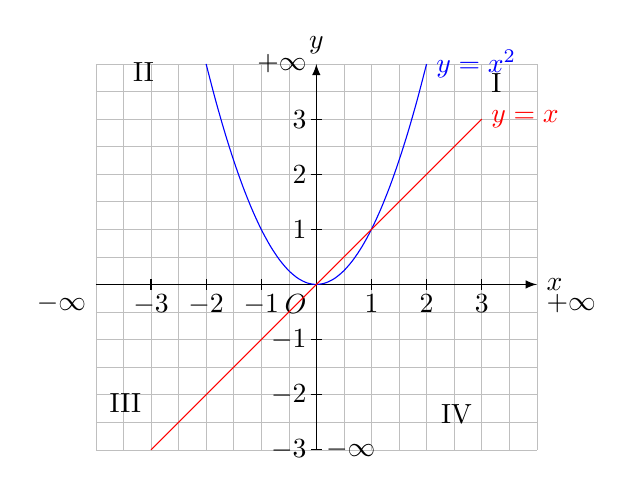
\begin{tikzpicture}[>=latex, scale=0.7]
    % Grid
    \draw[xstep=0.5,ystep=0.5,gray!50,very thin] (-4,-3) grid (4,4);
    % Axes
    \draw[->] (-4,0) -- (4,0) node[right] {$x$};
    \draw[->] (0,-3) -- (0,4) node[above] {$y$};
    % Label x and y axes
    \foreach \x in {-3,-2,-1,1,2,3}
        \draw (\x,-0.1) -- (\x,0.1) node[below=2pt] {$\x$};
    \foreach \y in {-3,-2,-1,1,2,3}
        \draw (-0.1,\y) -- (0.1,\y) node[left=2pt] {$\y$};
    % Label infinity
    \node[below right] at (4,0) {$+\infty$};
    \node[left] at (0,4) {$+\infty$};
    \node[below left] at (-4,0) {$-\infty$};
    \node[right] at (0,-3) {$-\infty$};
    % Label quarters
    \node[below left] at (0,0) {$O$};
    \node[below right] at (3,4) {I};
    \node[above right] at (-3.5,3.5) {II};
    \node[above left] at (-3,-2.5) {III};
    \node[below left] at (3,-2) {IV};
    % Plot y=x^2
    \draw[domain=-2:2,smooth,variable=\x,blue] plot ({\x},{\x*\x}) node[right] {$y=x^2$};
    % Plot y=x
    \draw[domain=-3:3,smooth,variable=\x,red] plot ({\x},{\x}) node[right] {$y=x$};
\end{tikzpicture}
\end{minipage}\\
To explore Polynomial functions along with their powers, functions, special names, graphs, domains, ranges, and end behaviors (whether they are decreasing or increasing) as well as leading terms, refer to the \href{run:./Unit\%201\%20-\%20Polynomial\%20Functions/Polynomial.tex}{Polynomial.tex} file.

\end{center}




\section*{Understanding Function Properties}

\subsection*{Even and Odd Degree Functions}

\textbf{Even Degree Functions:} Functions with even degrees have polynomial expressions where the highest power of the variable $x$ is an even number. These functions open upwards or downwards, and exhibit symmetry about the $y$-axis.

\textbf{Odd Degree Functions:} Functions with odd degrees have polynomial expressions where the highest power of the variable $x$ is an odd number. These functions open upwards or downwards, and exhibit symmetry about the origin.

\begin{center}
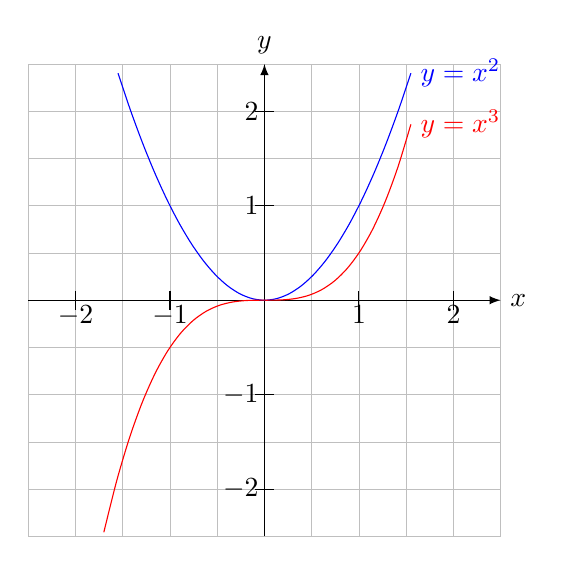
\begin{tikzpicture}[>=latex, scale=1.2]
  % Grid
  \draw[xstep=0.5,ystep=0.5,gray!50,very thin] (-2.5,-2.5) grid (2.5,2.5);
  % Axes
  \draw[->] (-2.5,0) -- (2.5,0) node[right] {$x$};
  \draw[->] (0,-2.5) -- (0,2.5) node[above] {$y$};
  % Labels
  \foreach \x in {-2,-1,1,2}
      \draw (\x,-0.1) -- (\x,0.1) node[below=2pt] {$\x$};
  \foreach \y in {-2,-1,1,2}
      \draw (-0.1,\y) -- (0.1,\y) node[left=2pt] {$\y$};
  % Even function
  \draw[domain=-1.55:1.55,smooth,variable=\x,blue] plot ({\x},{\x*\x}) node[right] {$y=x^2$};
  % Odd function
  \draw[domain=-1.70:1.55,smooth,variable=\x,red] plot ({\x},{0.5*\x*\x*\x}) node[right] {$y=x^3$};
\end{tikzpicture}
\end{center}

\subsection*{Understanding End Behavior}

\textbf{End Behavior:} Refers to the behavior of a function as $x$ approaches positive or negative infinity. 

\textbf{Describing End Behaviors:} End behaviors are described in terms of what happens to the function values as $x$ goes to positive or negative infinity.

\begin{center}
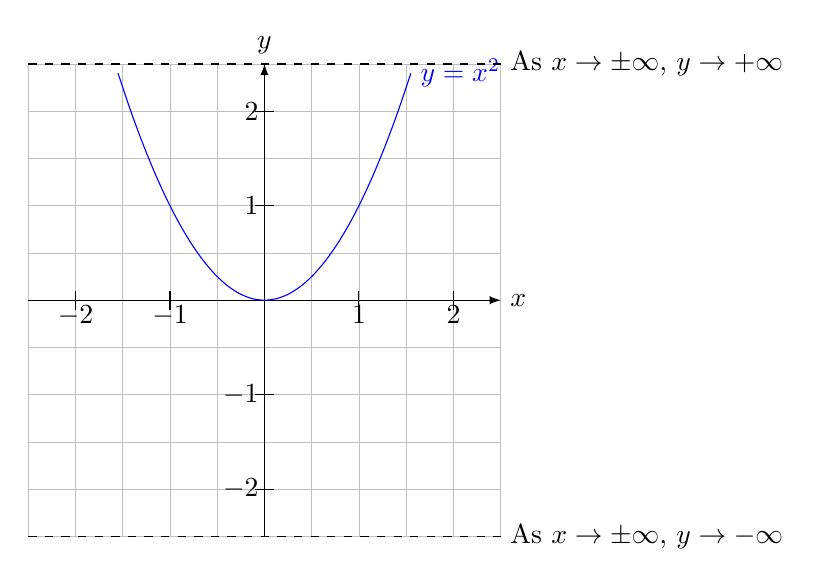
\begin{tikzpicture}[>=latex, scale=1.2]
  % Grid
  \draw[xstep=0.5,ystep=0.5,gray!50,very thin] (-2.5,-2.5) grid (2.5,2.5);
  % Axes
  \draw[->] (-2.5,0) -- (2.5,0) node[right] {$x$};
  \draw[->] (0,-2.5) -- (0,2.5) node[above] {$y$};
  % Labels
  \foreach \x in {-2,-1,1,2}
      \draw (\x,-0.1) -- (\x,0.1) node[below=2pt] {$\x$};
  \foreach \y in {-2,-1,1,2}
      \draw (-0.1,\y) -- (0.1,\y) node[left=2pt] {$\y$};
  % Even function
  \draw[domain=-1.55:1.55,smooth,variable=\x,blue] plot ({\x},{\x*\x}) node[right] {$y=x^2$};
  % End behaviors
  \draw[dashed] (-2.5,2.5) -- (2.5,2.5) node[right] {As $x \rightarrow \pm\infty$, $y \rightarrow +\infty$};
  \draw[dashed] (-2.5,-2.5) -- (2.5,-2.5) node[right] {As $x \rightarrow \pm\infty$, $y \rightarrow -\infty$};
\end{tikzpicture}
\end{center}

\subsection*{Properties of Power Functions}

\textbf{Domain and Range:} 
For power functions, the domain is all real numbers ($x \in \mathbb{R}$), and the range depends on whether the function is even or odd.

\textbf{Symmetry:} Power functions exhibit symmetry properties based on whether they are even or odd functions. 

\subsubsection{Deriving Polynomial Functions from Data:}

\begin{table}[h]
    \centering
    \begin{tabular}{|c|c|c|}
    \hline
        \rowcolor[HTML]{EFEFEF}
        $x$ & $y$ & $\Delta f(x)$ \\
        \hline
        1 & 1 & $2-1$\\
        \hline
        2 & 2 & \\
        \hline
        3 & 3 & \\
        \hline
        4 & 4 & $\vdots$ \\
        \hline
        $\vdots$ & $\vdots$ & $\vdots$\\
        \hline
        $m-1$ & $m-1$ & $m-(m-1)$\\
        \hline
        $m$ & $m$ & $m+1-m$\\
        \hline
        $m+1$ & $m+1$ & \\
        \hline
    \end{tabular}
    \caption*{The set of first differences for a linear function remains constant.}
\end{table}

\newpage
\section*{Union and Intersection}
If $A=\{1,3,5,7,9\}$ and $B=\{2,3,5,7$,$\} , what are A \cup B$ and $A \cap B$ ?

We have
$$
\begin{aligned}
& A \cup B=\{1,2,3,5,7,9\} \\
& A \cap B=\{3,5,7\} \cdot 
\end{aligned}
$$


\def\firstcircle{(0,0) circle (1cm)}
\def\secondcircle{(0:1.5cm) circle (1cm)}

\colorlet{circle edge}{blue!50}
\colorlet{circle area}{blue!20}

\tikzset{
    filled/.style = {fill=circle area, draw=circle edge, thick},
    outline/.style = {draw=circle edge, thick},
    F/.style = {draw, inner sep=7mm, fit=(current bounding box),
                node contents={}}
}



\begin{center}
\end{center}

\begin{figure}[h]
    \centering
    \begin{minipage}[t]{0.45\linewidth} 
        \centering   
        \begin{tikzpicture}
            \draw[filled] \firstcircle node {$A$}
                          \secondcircle node {$B$};
            \node (a) [F];                 
            \node[below left] at (a.north east) {$A \cup B$};
        \end{tikzpicture}
        \caption{Presentation of sets union by Venn diagram}
        \label{fig:ven-1a}
    \end{minipage}
    \hfil
    \begin{minipage}[t]{0.45\linewidth}
        \centering
        \begin{tikzpicture}
            \begin{scope}
                \clip \firstcircle;
                \fill[filled] \secondcircle;
            \end{scope}
            \draw[outline] \firstcircle node {$A$};
            \draw[outline] \secondcircle node {$B$};
            \node (a) [F];
            \node[below left] at (a.north east) {$A \cap B$};
        \end{tikzpicture}
        \caption{Presentation of sets intersection by Venn diagram}
        \label{fig:ven-1b}
    \end{minipage}% end of subfloat
\end{figure}


Feel free to learn more in \href{https://brilliant.org/wiki/sets-union-and-intersection-easy/#:~:text=The%20union%20of%202%20sets,the%20symbol%20is%20%E2%88%AAnion.}{Union and intersections}

\subsection{Characteristics of Polynomial Function}

A general note: Terminology of polynomial functions:\\
\begin{figure}[h]
    \centering
    \includegraphics[width=0.6\textwidth]{imgs/polynomial.jpg}
\end{figure}\\
Finite Differences: The nth differences for a polynomial of degree n will all
be the same, and this common difference will be equal to the product of n!
and the leading coefficient $(a_n)$.
\begin{align*}
\text{Common Difference} &= a_nn! (a_n \times n!)\\
&= a_n[n \times (n-1) \times (n-2) \times \cdots \times 3 \times 2 \times 1]
\end{align*}
where, 
\begin{itemize}
    \item \(a_n\) represents the \(n\)th term of the arithmetic sequence.
    \item \(n!\) represents the factorial of \(n\), which is the product of all positive integers up to \(n\). For example, \(5! = 5 \times 4 \times 3 \times 2 \times 1\).
\end{itemize}

\subsubsection*{Example:}The finite differences are taken for a polynomial function, and the 6th differences are found to all be -2880. What was the
leading coefficient of the polynomial function.
Given:
\[
\text{Common Difference} = -2880 = a \times 6!
\]

We are trying to find the value of \(a\). So, let's solve for \(a\):

\[a = \frac{-2880}{6!} = \frac{-2880}{720} = -4\]

So, the value of \(a\) is indeed \(-4\).
\subsubsection{Anatomy of a Polynomial Function:}
\begin{figure}[ht]
    \centering
    \includegraphics[width=0.6\textwidth]{imgs/anatomyofapolynomialfunction.png}
\end{figure}


To learn more about the characteristics of polynomial functions, you can visit the following link: \href{https://mathematicalmysteries.org/characteristics-of-polynomials/}{Characteristics of Polynomial Function}.






















\newpage
Domain \& Range, Absolute value (definition), Polynomial functions, Composite and Inverse. \\ 

\textbf{Absolute value:} $f(x)= |x|$, the definition that "x" is from the origin on the number line. \\ 
In general:\\
$$
|f(x)|=
\begin{cases}
f(x) &, f(x) \ge 0\\
-f(x) &, f(x) < 0
\end{cases}
$$
\\
\textbf{Odd functions:} A function $f(x)$ is odd if $f(-x)= -f(x)$. Symmetric about the origin or reflection along both the x and y axis. \\ \\

$\quad f(x)=-2x^3+x$, is an odd function since $f(-x)=-2(-x)^3+(-x)$ \\ \\ 

\textbf{Note:}$f(-x)=-f(x)$ \\ 
For polynomial functions, the function is an odd function if all exponents are odd. \\ \\ 


\textbf{Even functions:} A function $f(x)$ is even if $f(-x)=f(x)$. Symmetric about the y-axis. \\ \\ 

i.e $\quad f(x)=3x^4+2x^2-2$, is an even function since function if all the exponents are even. \\ \\ 

\end{document}
